\documentclass[10pt,UTF8]{book} %% ctexart

\title{\textbf{数据库系统基础}}
\author{钱锋\thanks{Email: strik0r.qf@gmail.com}${}^,$\thanks{
    西北工业大学软件学院, School of Software, Northwestern Polytechnical University, 西安 710072
}}

\usepackage{ctex}
\usepackage{graphicx}
\usepackage[toc]{multitoc}
\usepackage{booktabs}
\usepackage{longtable}
\usepackage{amsthm, amssymb, amsmath, mathrsfs, mhchem}
\usepackage{tikz,circuitikz}
\usetikzlibrary{decorations.markings, angles, quotes}
\usetikzlibrary{shapes,arrows.meta,positioning}
\usepackage{tikz-cd}
\usepackage{pgfplots}
\usepackage{tikz-3dplot}
\usepackage{extpfeil}
\usepackage{diagbox}
\usepackage{float}
\usepackage{hyperref}
\hypersetup{hidelinks,
    colorlinks = true,
    allcolors = black,
    pdfstartview = Fit,
    breaklinks = true}
\usepackage{caption}
\usepackage{enumitem}
\usepackage{siunitx}
\usepackage{subcaption}

\usepackage{fancyhdr} % 用于自定义页眉页脚


% 设置页眉页脚样式
\fancypagestyle{plain}{%
    \fancyhf{} % 清空页眉页脚
    \fancyhead[RO,LE]{·\thepage·} % 页眉显示页码, RO表示奇数页右侧, LE表示偶数页左侧
    \fancyhead[LO]{\nouppercase{\rightmark}} % 页眉显示小节标题, LO表示奇数页左侧
    \fancyhead[RE]{\nouppercase{\leftmark}} % 页眉显示章节标题, RE表示偶数页右侧
    \renewcommand{\headrulewidth}{0.4pt} % 设置页眉横线的宽度
    \renewcommand{\footrulewidth}{0pt} % 取消页脚横线
}

\renewcommand{\headrule}{\hrule width\textwidth height\headrulewidth\vskip-\headrulewidth}

% % 取消奇偶页的页眉偏移
% \fancyhfoffset[RO,LE]{0pt}

% % 取消奇偶页的页眉偏移
% \fancyhfoffset[RO,LE]{0pt}

% 定义取消页眉的命令
\newcommand{\cancelheader}{%
    \fancyhead{} % 清空页眉
    \renewcommand{\headrulewidth}{0pt} % 取消页眉横线
    \renewcommand{\footrulewidth}{0pt} % 设置页脚横线的宽度
}

\renewcommand{\chaptermark}[1]{\markboth{第 \thechapter 章 \hspace{1em} #1}{}}
\renewcommand{\sectionmark}[1]{\markright{\thesection \, #1}}
\usepackage{titlesec} % 定义标题样式

% 设置 chapter 标题样式
\titleformat{\chapter}[hang]{\centering\heiti\Large\bfseries}{第\,\thechapter\,章}{1em}{}

% 定义 section 标题格式
\titleformat{\section}[hang]{\heiti\centering\large\bfseries}{\thesection}{1em}{}

% 定义 subsection 标题格式
\titleformat{\subsection}[hang]{\heiti\bfseries}{\textbf{\thesubsection}}{1em}{}

% 定义 subsubsection 标题格式
\setcounter{secnumdepth}{3}
\renewcommand\thesubsubsection{\arabic{subsubsection}.}
\titleformat{\subsubsection}[hang]{\kaishu}{\quad\quad\thesubsubsection\,\,}{0em}{}

% % 重新定义 textbf
% \let\oldtextbf\textbf
% \renewcommand{\textbf}[1]{{\heiti\oldtextbf{#1}}}

% % 在导言区重新定义 \normalsize 命令
% \makeatletter
% \renewcommand\normalsize{%
%    \@setfontsize\normalsize{10.5pt}{12pt}%
%    \abovedisplayskip 8\p@ \@plus2\p@ \@minus5\p@
%    \abovedisplayshortskip \z@ \@plus3\p@
%    \belowdisplayshortskip 6\p@ \@plus3\p@ \@minus3\p@
%    \belowdisplayskip \abovedisplayskip
%    \let\@listi\@listI}
% \makeatother



% 设置页边距和对齐
% \usepackage[
%     paperwidth=185mm,
%     paperheight=260mm,
%     top=35mm,
%     bottom=25mm,
%     left=18mm,
%     right=18mm,
%     footskip=15mm % 通过这里的值来调整页脚与正文内容的垂直距离
% ]{geometry}

\usepackage[
    paperwidth=210mm,
    paperheight=297mm,
    top=40mm,
    bottom=31.8mm,
    left=25.4mm,
    right=25.4mm,
    footskip=15mm % 通过这里的值来调整页脚与正文内容的垂直距离
]{geometry}

% \usepackage[
%     paperwidth=195mm,
%     paperheight=270mm,
%     top=40mm,
%     bottom=25mm,
%     left=23.5mm,
%     right=23.5mm,
%     footskip=15mm % 通过这里的值来调整页脚与正文内容的垂直距离
% ]{geometry}
\usepackage{mdframed}
\mdfsetup{
  linewidth=0.4pt,
  frametitlebackgroundcolor=white, % 或者 transparent
  frametitlefont=\heiti\bfseries,
  frametitleaboveskip=10pt,
  frametitlebelowskip=5pt,
  frametitlealignment=\raggedright % 新增此行
}
\usepackage{fontspec}
% 设置 Menlo 字体
\setmonofont{Menlo}
\usepackage{fancyvrb}
\usepackage{xcolor}
\usepackage{listings}

% \definecolor{string}{HTML}{067D17}
% \definecolor{comment}{HTML}{8C8C8C}
% \definecolor{keyword}{HTML}{0033B3}
% \definecolor{class_field}{HTML}{871094}

\lstset{breaklines}
%这条命令可以让LaTeX自动将长的代码行换行排版
\lstset{extendedchars=false}
%这一条命令可以解决代码跨页时,章节标题,页眉等汉字不显示的问题
\lstset{escapeinside={(*}{*)}}

\lstset{
    basicstyle=\small\ttfamily\heiti,
    numbers=left,
    numberstyle=\scriptsize\fontspec{Menlo}, % 使用 Menlo 字体
    stepnumber=1,
    numbersep=8pt,
    frame=leftline,
    xleftmargin=2em, % 调整代码块的左边界
    framexleftmargin=0pt, % 调整边框的位置
    breaklines=true,
    % postbreak=\mbox{\textcolor{red}{$\hookrightarrow$}\space},
    % keywordstyle=\bfseries\color{keyword},          % keyword style
    % commentstyle=\heiti\color{comment},       % comment style
    % stringstyle=\color[HTML]{067D17},
    showstringspaces=false,
    % string literal style
    % escapeinside={\%*}{*)},            % if you want to add LaTeX within your code
    % morekeywords={}               % if you want to add more keywords to the set
}

\usepackage{smartdiagram} % 表格对角线
\everymath{\displaystyle}
\usepackage{tasks}

\begin{document}
\newtheoremstyle{mytheoremstyle}
    {1.5ex}                                         % Space above
    {1.5ex}                                         % Space below
    {}                                              % Font for body
    {}                                              % Indent amount
    {\bfseries}                                     % Font for head
    {}                                              % Punctuation after head
    {0.5em plus 0.2em minus 0.1em}                  % Space after head
    {\thmname{#1}\thmnumber{ #2}.\thmnote{ (#3).}}

\theoremstyle{mytheoremstyle}
\newtheorem{definition}{定义}[section]
\newtheorem{example}{例}[section]
\newtheorem{exercise}{习题}[section]
\newtheorem{code}{程序清单}[section]
\newtheorem*{result}{运行结果}

\newtheoremstyle{my2theoremstyle}
    {1.5ex}                                         % Space above
    {1.5ex}                                         % Space below
    {\kaishu}                                              % Font for body
    {}                                              % Indent amount
    {\bfseries}                                     % Font for head
    {}                                              % Punctuation after head
    {0.5em plus 0.2em minus 0.1em}                  % Space after head
    {\thmname{#1}\thmnumber{ #2}.\thmnote{ (#3).}}

\theoremstyle{my2theoremstyle}
\newtheorem{thm}{定理}[section]
\newtheorem{law}{定律}[section]
\newtheorem{educt}{推论}
\newtheorem{prop}{命题}
\newtheorem{lemma}{引理}
\newtheorem{axiom}{公理}
\newtheorem{property}{性质}

\newtheoremstyle{my4theoremstyle}
    {1.5ex}                                         % Space above
    {1.5ex}                                         % Space below
    {}                                              % Font for body
    {}                                              % Indent amount
    {\bfseries}                                     % Font for head
    {}                                              % Punctuation after head
    {0.5em plus 0.2em minus 0.1em}                  % Space after head
    {\thmname{#1}.}

\theoremstyle{my4theoremstyle} \newtheorem*{sol}{解}

\newtheoremstyle{my3theoremstyle}
    {1.5ex}                                         % Space above
    {1.5ex}                                         % Space below
    {}                                              % Font for body
    {}                                              % Indent amount
    {\kaishu}                                       % Font for head
    {}                                              % Punctuation after head
    {0.5em plus 0.2em minus 0.1em}                  % Space after head
    {\thmname{#1}\thmnumber{ #2}.\thmnote{ (#3).}}

\theoremstyle{my3theoremstyle} \newtheorem*{remark}{注}
\newtheorem*{cmt}{评注}
% 使用 IEEE 样式
\ctikzset{logic ports=ieee}
\pagestyle{empty}
\begin{titlepage}
    \thispagestyle{empty}
    \centering
        \vspace*{2cm}
        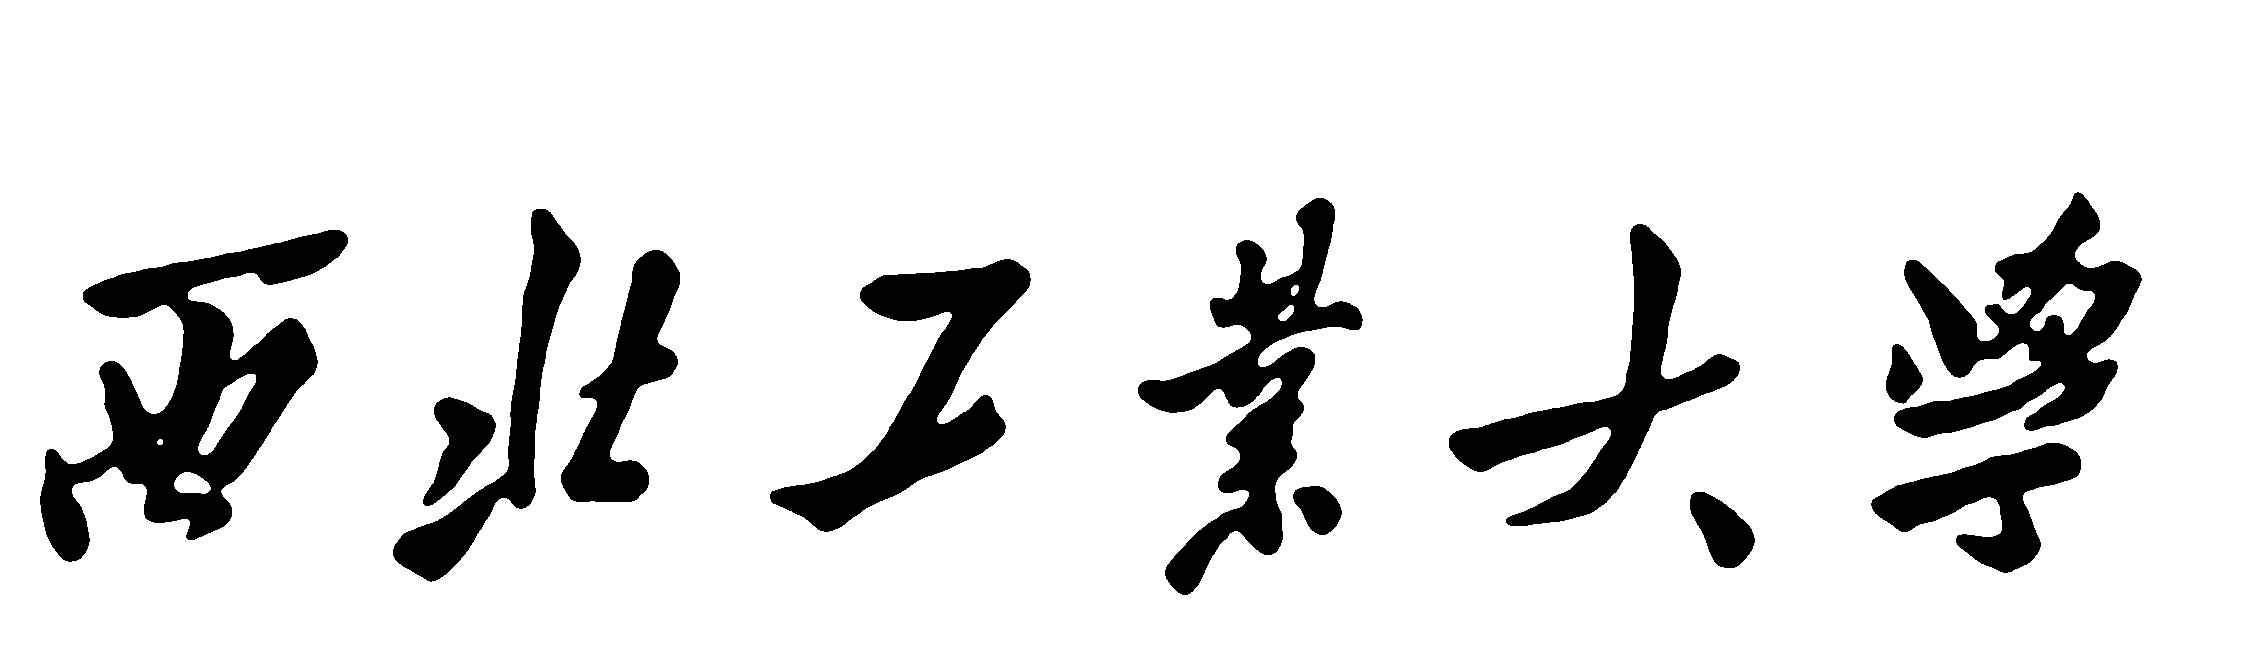
\includegraphics[width=0.5\textwidth]{pic/npu_2.png}\par
        \vspace{1em}
        
\includegraphics[width=0.5\textwidth]{pic/npu_1.png}\par
    \vspace{1em}
        \begin{center}
            \Huge \heiti \textbf{数据库系统基础}

            Fundamentals of Database Systems
        \end{center}
        \vspace{17em}
        \begin{center}
        \songti
        \kaishu 软件学院 \, \heiti\textbf{钱锋} \quad \songti 编
        \vspace{0.5em}

    \today
    \end{center}
\end{titlepage}
\cleardoublepage
\maketitle
\cleardoublepage

\frontmatter
\newpage
\pagestyle{plain}
\makeatother

% \input{丛书前言.tex}

% \chapter{课程概述}
% \thispagestyle{empty}

% \newpage
% \thispagestyle{empty}

% 设置目录页的页码格式
\pagenumbering{roman} % 切换回罗马数字页码
\addtocontents{toc}{\protect\thispagestyle{empty}}
\pagestyle{plain}
{\tableofcontents}
\newpage
\thispagestyle{empty}
\cleardoublepage % 确保正文从奇数页开始


% 设置章节标题页的页眉和页脚为空白页样式
\makeatletter
\let\ps@plain\ps@empty
\makeatother

\mainmatter
\chapter{数据库简介}
% \section{数据库技术的起源与发展}

% \subsection{数据管理技术发展阶段}

\section{数据库与数据库管理系统}

\subsection{数据库的四个基本概念}

\textbf{数据} (data) 是描述客观事物的符号记录.



\textbf{数据库} (database) 
% 是相关数据的集合, 可以通过\textbf{数据} (data) 来记录我们
% 所知的现实情况, 并赋予他们隐含的含义. 数据库具有以下三个隐含属性:
% \begin{itemize}[itemsep=0pt]
%     \item 数据库\textbf{表示现实的某个方面}: 有时将现实世界的某个方面称之
%     为\textbf{微观世界} (miniworld) 或者\textbf{论域} 
%     (universe of discourse, UoD). 微观世界的改变将会反映在数据库中.
%     \item 数据库是具有某种内在含义的、逻辑上协调一致的数据的集合.
%     \item 数据库是处于特定目的而设计、构建以及填充数据的.
% \end{itemize}
% 概括地说, 
% 数据库
是长期存储在计算机内部的、有组织的、可共享的大量数据的集合, 数据库中的数据
按照一定的数据模型组织、描述和储存, 具有较小的冗余度、较高的数据独立性和易拓展性,
并可为各种用户所共享.

% 数据库可以具有任意的规模性和复杂性.



\textbf{数据库管理系统} (database management system, DBMS) 是一个用于定义、构造和
操作数据库和自爱不同的用户与应用之间共享数据库的通用软件系统
(general-purpose software system). 它允许用户创建和维护数据库.
% \begin{itemize}[itemsep=0pt]
%     \item \textbf{定义} (define): 为将要存储在数据库中的数据指定数据类型、结构和约束条件.
%     数据库定义和描述信息, 即\textbf{元数据} (meta-data) 也是由 DBMS 以数据库目录或字典
%     的形式存储的.
%     \item \textbf{构造} (construct): 在 DBMS 的控制之下将数据存储在某种存储媒介上.
%     \item \textbf{操作} (manipulate): 包括查询数据库以检索特定的数据、更新数据库以反映
%     微观世界的改变以及通过数据生成报表等.
%     \item \textbf{共享} (share): 允许多个用户和程序同时访问数据库.
%     \item \textbf{保护} (protection): 例如防止软硬件故障的系统保护以及防止未经授权
%     或恶意访问数据库的安全保护.
%     \item \textbf{维护} (maintain): 使得数据库系统可以在长时间内随着需求的变化而不断演化.
% \end{itemize}
% 应用程序 (application program) 通过向 DBMS 发送查询或数据请求来访问数据库. \textbf{查询}
% (query) 通过会执行数据检索; 而\textbf{事务} (transcation) 则用于执行从数据库中读取数据或者
% 将数据写入数据库中.

\textbf{数据库系统} (database system) 是由数据库、DBMS、应用程序 (application program)
和数据库管理员 (database administer, DBA) 组成的存储、管理、处理和维护数据的系统.

\begin{figure}[H]
    \centering
    

\tikzset{every picture/.style={line width=0.75pt}} %set default line width to 0.75pt        

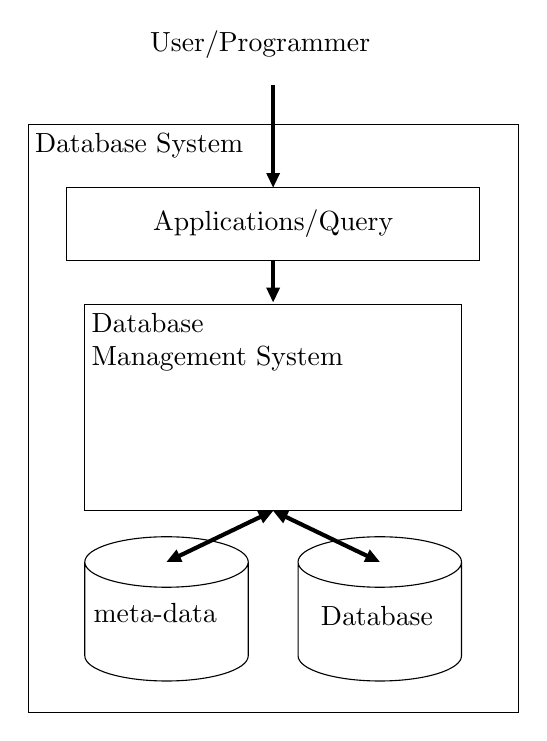
\begin{tikzpicture}[x=0.75pt,y=0.75pt,yscale=-1,xscale=1]
%uncomment if require: \path (0,427); %set diagram left start at 0, and has height of 427

%Shape: Rectangle [id:dp01515462542343704] 
\draw   (100,63.5) -- (336,63.5) -- (336,346.5) -- (100,346.5) -- cycle ;
%Shape: Rectangle [id:dp9866371707331819] 
\draw   (127.25,150) -- (308.75,150) -- (308.75,249.5) -- (127.25,249.5) -- cycle ;
%Flowchart: Magnetic Disk [id:dp6221057101121902] 
\draw   (206,274.16) -- (206,319.34) .. controls (206,326.05) and (188.37,331.5) .. (166.63,331.5) .. controls (144.88,331.5) and (127.25,326.05) .. (127.25,319.34) -- (127.25,274.16)(206,274.16) .. controls (206,280.88) and (188.37,286.33) .. (166.63,286.33) .. controls (144.88,286.33) and (127.25,280.88) .. (127.25,274.16) .. controls (127.25,267.45) and (144.88,262) .. (166.63,262) .. controls (188.37,262) and (206,267.45) .. (206,274.16) -- cycle ;
%Flowchart: Magnetic Disk [id:dp8335122842260207] 
\draw   (308.75,274.16) -- (308.75,319.34) .. controls (308.75,326.05) and (291.12,331.5) .. (269.38,331.5) .. controls (247.63,331.5) and (230,326.05) .. (230,319.34) -- (230,274.16)(308.75,274.16) .. controls (308.75,280.88) and (291.12,286.33) .. (269.38,286.33) .. controls (247.63,286.33) and (230,280.88) .. (230,274.16) .. controls (230,267.45) and (247.63,262) .. (269.38,262) .. controls (291.12,262) and (308.75,267.45) .. (308.75,274.16) -- cycle ;
%Straight Lines [id:da6416908174630893] 
\draw [line width=1.5]    (218,44.5) -- (218,89.75) ;
\draw [shift={(218,93.75)}, rotate = 270] [fill={rgb, 255:red, 0; green, 0; blue, 0 }  ][line width=0.08]  [draw opacity=0] (6.97,-3.35) -- (0,0) -- (6.97,3.35) -- cycle    ;
%Straight Lines [id:da39888614015754065] 
\draw [line width=1.5]    (218,128.75) -- (218,145) ;
\draw [shift={(218,149)}, rotate = 270] [fill={rgb, 255:red, 0; green, 0; blue, 0 }  ][line width=0.08]  [draw opacity=0] (6.97,-3.35) -- (0,0) -- (6.97,3.35) -- cycle    ;
%Straight Lines [id:da49744353352368653] 
\draw [line width=1.5]    (221.61,251.23) -- (265.77,272.43) ;
\draw [shift={(269.38,274.16)}, rotate = 205.64] [fill={rgb, 255:red, 0; green, 0; blue, 0 }  ][line width=0.08]  [draw opacity=0] (6.97,-3.35) -- (0,0) -- (6.97,3.35) -- cycle    ;
\draw [shift={(218,249.5)}, rotate = 25.64] [fill={rgb, 255:red, 0; green, 0; blue, 0 }  ][line width=0.08]  [draw opacity=0] (6.97,-3.35) -- (0,0) -- (6.97,3.35) -- cycle    ;
%Straight Lines [id:da2751170640767556] 
\draw [line width=1.5]    (214.39,251.23) -- (170.23,272.43) ;
\draw [shift={(166.63,274.16)}, rotate = 334.36] [fill={rgb, 255:red, 0; green, 0; blue, 0 }  ][line width=0.08]  [draw opacity=0] (6.97,-3.35) -- (0,0) -- (6.97,3.35) -- cycle    ;
\draw [shift={(218,249.5)}, rotate = 154.36] [fill={rgb, 255:red, 0; green, 0; blue, 0 }  ][line width=0.08]  [draw opacity=0] (6.97,-3.35) -- (0,0) -- (6.97,3.35) -- cycle    ;

% Text Node
\draw (102,66.5) node [anchor=north west][inner sep=0.75pt]   [align=left] {Database System};
% Text Node
\draw    (118.5,93.75) -- (317.5,93.75) -- (317.5,128.75) -- (118.5,128.75) -- cycle  ;
\draw (218,111.25) node   [align=left] {\begin{minipage}[lt]{132.6pt}\setlength\topsep{0pt}
\begin{center}
Applications/Query
\end{center}

\end{minipage}};
% Text Node
\draw (129.25,153) node [anchor=north west][inner sep=0.75pt]   [align=left] {Database \\Management System};
% Text Node
\draw (130.25,293) node [anchor=north west][inner sep=0.75pt]   [align=left] {meta-data};
% Text Node
\draw (239.75,294) node [anchor=north west][inner sep=0.75pt]   [align=left] {Database};
% Text Node
\draw (157.5,17) node [anchor=north west][inner sep=0.75pt]   [align=left] {User/Programmer};


\end{tikzpicture}
\caption{一种简化的数据库系统环境}
\end{figure}

\subsection{数据管理技术的发展}





虽然数据库是当前数据管理最有效的方式之一, 在数据库技术出现之前, 数据管理还
经历了两个阶段, 分别是手工管理阶段和文件系统管理阶段.

% \begin{itemize}[itemsep=0pt]
%     \item \textbf{手工管理阶段}
%     \item \textbf{文件系统管理阶段}
%     \item \textbf{数据库系统管理阶段}
%     \item \textbf{大数据管理系统}
% \end{itemize}

\begin{table}[H]
    \centering
    \caption{不同数据管理技术发展阶段的特点}
    \begin{tabular}{p{0.1\textwidth}|p{0.1\textwidth}p{0.1\textwidth}p{0.15\textwidth}p{0.2\textwidth}p{0.2\textwidth}}
        \hline
        \textbf{发展阶段} & \textbf{年代背景} & \textbf{应用背景} & \textbf{硬件条件} & \textbf{软件条件} & \textbf{数据管理} \\ 
        \hline
        \textbf{手工管理} & 1950s 之前 & 科学计算 & 打孔卡片、磁带; \newline 没有磁盘 & 没有操作系统和专门的数据管理软件; \newline 数据交互按照批处理方式进行 & 数据与程序相互依赖; \newline 数据没有共享 \\ 
        \hline
        \textbf{文件管理} & 1950s-60s & 科学计算; \newline 数据管理 & 磁盘、磁鼓 & 操作系统下产生文件系统; \newline 数据实时在线处理 & 数据文件相互独立; \newline 数据共享困难, 冗余 \\ 
        \hline
        \textbf{数据库} & 1960s 之后 & 大规模数据管理 & 大容量磁盘 & 产生了专门的数据管理软件——数据库管理系统, 以满足不同的场景应用需求 & 实现数据的共享、透明 \\ 
        \hline
    \end{tabular}
\end{table}
\begin{figure}[H]
    \centering
    \begin{minipage}{0.3\textwidth}
        \centering
        \begin{tikzpicture}[scale=0.7]
            \draw (0,0) node{程序 1} ellipse (1cm and 0.5cm);
            \draw (1.5,0) -- (3.5,0);
            \draw (5,0) node{数据 1} ellipse (1cm and 0.5cm);
    
            \draw (0,-1.5) node{程序 2} ellipse (1cm and 0.5cm);
            \draw (1.5,-1.5) -- (3.5,-1.5);
            \draw (5,-1.5) node{数据 2} ellipse (1cm and 0.5cm);
    
            \draw (0,-3) node{程序 3} ellipse (1cm and 0.5cm);
            \draw (1.5,-3) -- (3.5,-3);
            \draw (5,-3) node{数据 3} ellipse (1cm and 0.5cm);
        \end{tikzpicture}
        \subcaption{手工管理阶段的程序和数据基本是一一对应的, 没有数据共享}
    \end{minipage}
    \begin{minipage}{0.5\textwidth}
        \centering
        \begin{tikzpicture}[scale=0.8]
            \draw (-1,0) node{程序 1} ellipse (1cm and 0.5cm);
            \draw (0,0) -- (1.5,-1.5);
            \draw (3.5,-1.5) -- (5,0);
            \draw (6,0) node{数据 1} ellipse (1cm and 0.5cm);
    
            \draw (-1,-1.5) node{程序 2} ellipse (1cm and 0.5cm);
            \draw (0, -1.5) -- (1.5,-1.5);
            \draw (3.5,-1.5) -- (5,-1.5);
            \draw (6,-1.5) node{数据 2} ellipse (1cm and 0.5cm);
    
            \draw (-1,-3) node{程序 3} ellipse (1cm and 0.5cm);
            \draw (0, -3) -- (1.5,-1.5);
            \draw (3.5,-1.5) -- (5,-3);
            \draw (6,-3) node{数据 3} ellipse (1cm and 0.5cm);
    
            \draw (2.5,-1.5) node{文件系统} ellipse (1cm and 0.5cm);
        \end{tikzpicture}
        \subcaption{在文件系统阶段, 数据文件相互独立但是共享困难}
    \end{minipage}

    \vspace{1em}

    \begin{minipage}{\textwidth}
        \centering
        \begin{tikzpicture}[scale=0.8]
            \draw (-1.5,0) node{程序 1} ellipse (1cm and 0.5cm);
            \draw (-0.5,0) -- (0.5,-1.5);
    
            \draw (-1.5,-1.5) node{程序 2} ellipse (1cm and 0.5cm);
            \draw (-0.5, -1.5) -- (0.5,-1.5);
            \draw (4.5,-1.5) -- (6,-1.5);
            \draw (7,-1.5) node{数据库} ellipse (1cm and 0.5cm);
    
            \draw (-1.5,-3) node{程序 3} ellipse (1cm and 0.5cm);
            \draw (-0.5, -3) -- (0.5,-1.5);
    
            \draw (2.5,-1.5) node{数据库管理系统} ellipse (2cm and 0.5cm);
        \end{tikzpicture}
        \subcaption{数据库系统阶段实现了焦点分离}
    \end{minipage}
    \caption{数据库技术的不同阶段的特点}
\end{figure}

\section{数据模型 \quad 数据库系统的模式架构}

\subsection{数据模型分类}

数据模型分为\textbf{概念数据模型} (conceptual data model)、
\textbf{物理数据模型} (physical data model) 和介于二者之间的\textbf{实现数据模型}
(implementational data model).
\begin{itemize}[itemsep=0pt]
    \item 概念数据模型按照用户的观点来为数据和信息进行建模.
    \item 物理数据模型描述了在计算机存储介质上存储数据的细节.
\end{itemize}

概念数据模型使用实体、属性和关系等概念来进行建模. 我们会在第 \ref{chap: ER model} 章中介绍
\textbf{实体—关系模型} (entity-relationship model, ER model) 和这些有关的概念.

实现数据模型包括广泛使用的\textbf{关系数据模型} (relational data model) 以及
已经过时的网状模型 (network model) 和层次模型 (hierachical model), 还有一些更高级的实现
数据模型的新家族成员, 例如\textbf{对象数据模型} (object data model).

\subsection{数据库系统的模式架构}

\begin{figure}[H]
    \centering
    % 图的内容


    \tikzset{every picture/.style={line width=0.75pt}} %set default line width to 0.75pt        

    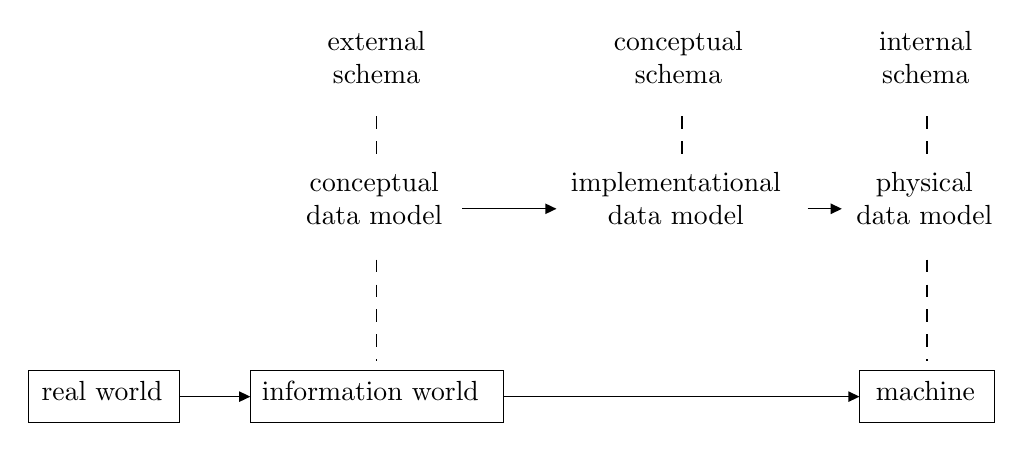
\begin{tikzpicture}[x=0.75pt,y=0.75pt,yscale=-1,xscale=1]
    %uncomment if require: \path (0,300); %set diagram left start at 0, and has height of 300
    
    %Straight Lines [id:da6888236647331167] 
    \draw  [dash pattern={on 4.5pt off 4.5pt}]  (194,154.5) -- (194,203.5) ;
    %Straight Lines [id:da5140114108378135] 
    \draw  [dash pattern={on 4.5pt off 4.5pt}]  (459,154.5) -- (459,203.5) ;
    %Straight Lines [id:da9015634759886653] 
    \draw    (99,220.5) -- (130,220.5) ;
    \draw [shift={(133,220.5)}, rotate = 180] [fill={rgb, 255:red, 0; green, 0; blue, 0 }  ][line width=0.08]  [draw opacity=0] (5.36,-2.57) -- (0,0) -- (5.36,2.57) -- cycle    ;
    %Straight Lines [id:da15947017273673214] 
    \draw    (255,220.5) -- (423.5,220.5) ;
    \draw [shift={(426.5,220.5)}, rotate = 180] [fill={rgb, 255:red, 0; green, 0; blue, 0 }  ][line width=0.08]  [draw opacity=0] (5.36,-2.57) -- (0,0) -- (5.36,2.57) -- cycle    ;
    %Straight Lines [id:da12741905382504892] 
    \draw    (235,130) -- (277.5,130) ;
    \draw [shift={(280.5,130)}, rotate = 180] [fill={rgb, 255:red, 0; green, 0; blue, 0 }  ][line width=0.08]  [draw opacity=0] (5.36,-2.57) -- (0,0) -- (5.36,2.57) -- cycle    ;
    %Straight Lines [id:da8746216303282328] 
    \draw    (401.5,130) -- (415,130) ;
    \draw [shift={(418,130)}, rotate = 180] [fill={rgb, 255:red, 0; green, 0; blue, 0 }  ][line width=0.08]  [draw opacity=0] (5.36,-2.57) -- (0,0) -- (5.36,2.57) -- cycle    ;
    %Straight Lines [id:da5170374392849098] 
    \draw  [dash pattern={on 4.5pt off 4.5pt}]  (459,85.5) -- (459,107.5) ;
    %Straight Lines [id:da5715165373295344] 
    \draw  [dash pattern={on 4.5pt off 4.5pt}]  (341,85.5) -- (341,107.5) ;
    %Straight Lines [id:da7700125694774308] 
    \draw  [dash pattern={on 4.5pt off 4.5pt}]  (194,85.5) -- (194,107.5) ;
    
    % Text Node
    \draw    (26,208) -- (99,208) -- (99,233) -- (26,233) -- cycle  ;
    \draw (29,212) node [anchor=north west][inner sep=0.75pt]   [align=left] {\begin{minipage}[lt]{46.94pt}\setlength\topsep{0pt}
    \begin{center}
    real world
    \end{center}
    
    \end{minipage}};
    % Text Node
    \draw    (133,208) -- (255,208) -- (255,233) -- (133,233) -- cycle  ;
    \draw (136,212) node [anchor=north west][inner sep=0.75pt]   [align=left] {\begin{minipage}[lt]{80.39pt}\setlength\topsep{0pt}
    \begin{center}
    information world
    \end{center}
    
    \end{minipage}};
    % Text Node
    \draw    (426.5,208) -- (491.5,208) -- (491.5,233) -- (426.5,233) -- cycle  ;
    \draw (429.5,212) node [anchor=north west][inner sep=0.75pt]   [align=left] {\begin{minipage}[lt]{41.28pt}\setlength\topsep{0pt}
    \begin{center}
    machine
    \end{center}
    
    \end{minipage}};
    % Text Node
    \draw (156,111) node [anchor=north west][inner sep=0.75pt]   [align=left] {\begin{minipage}[lt]{53.19pt}\setlength\topsep{0pt}
    \begin{center}
    conceptual\\data model
    \end{center}
    
    \end{minipage}};
    % Text Node
    \draw (421,111) node [anchor=north west][inner sep=0.75pt]   [align=left] {\begin{minipage}[lt]{53.19pt}\setlength\topsep{0pt}
    \begin{center}
    physical\\data model
    \end{center}
    
    \end{minipage}};
    % Text Node
    \draw (283.5,111) node [anchor=north west][inner sep=0.75pt]   [align=left] {\begin{minipage}[lt]{79.84pt}\setlength\topsep{0pt}
    \begin{center}
    implementational\\data model
    \end{center}
    
    \end{minipage}};
    % Text Node
    \draw (166.5,43) node [anchor=north west][inner sep=0.75pt]   [align=left] {\begin{minipage}[lt]{39.02pt}\setlength\topsep{0pt}
    \begin{center}
    external\\schema
    \end{center}
    
    \end{minipage}};
    % Text Node
    \draw (303.25,43) node [anchor=north west][inner sep=0.75pt]   [align=left] {\begin{minipage}[lt]{52.06pt}\setlength\topsep{0pt}
    \begin{center}
    conceptual\\schema
    \end{center}
    
    \end{minipage}};
    % Text Node
    \draw (431.5,43) node [anchor=north west][inner sep=0.75pt]   [align=left] {\begin{minipage}[lt]{38.44pt}\setlength\topsep{0pt}
    \begin{center}
    internal\\schema
    \end{center}
    
    \end{minipage}};
    
    
    \end{tikzpicture}
    \caption{数据库系统的模式架构}
    \label{数据库系统的模式架构}
\end{figure}

数据库系统的\textbf{内模式} (internal schema) 属于数据库系统的\textbf{内层} (internal level),
它描述了数据库的物理存储结构, 使用物理数据模型.

\textbf{概念模式} (conceptual schema) 属于数据库系统的\textbf{概念层} (conceptual level),
它专注于描述实体、数据类型、关系、用户操作以及约束, 使用实现数据模型.

\textbf{外模式} (external schema) s呼吁数据库系统的\textbf{外层} (external level)
或\textbf{视图层} (view level), 它针对特定用户组来描述感兴趣的数据库的一部分, 并隐藏数据库的其他部分.

在不同的层次之间存在着\textbf{映射} (mapping), 外层—概念层映射实现外层与概念层的请求和结果之间的
转换, 概念层—内层映射则实现概念层与内层的请求和结果之间的转换.

\subsection{数据独立性}

\textbf{数据独立性} (data independence) 是指, 当改变数据库系统某一层上的模式时,
无需改变其上层的模式. 因此数据独立性又分为\textbf{逻辑数据独立性} (logical data independence)
和\textbf{物理数据独立性} (physical data independence).
当某一层的模式改变时, 数据独立性保证了更高层上的模式可以保持不变, 只需要更改两个层次之间的映射即可.
这为数据库的设计、使用和维护带来了极大的便利.

\chapter{实体—联系模型}
\label{chap: ER model}

\begin{example}
    CBA 赛事包括球队 (team)、球员 (player) 和比赛 (game) 的信息. 
    每个球队有唯一的编号 (tNo)、名称 (tName) 和所属城市 (tCity).
    每个球队有多名球员, 每名球员有唯一的编号 (pNo)、姓名 (pName)、位置
    (pPosition)、体重 (pWeight) 和年龄 (pAge).
    每场比赛有唯一的编号 (gNo)、日期 (gDate)、地点 (gLocation) 和主客场球队.
    每场比赛有多个球员参与, 每个球员在比赛中有特定的表现数据, 例如得分 (pgPoints)、
    助攻 (pgAssists) 和篮板 (pgRebounds).
    根据以上信息构造的满足数据需求的实体—联系 (ER) 模型 
    如图 \ref{example-er:team-player-game} 所示.
    \begin{figure}[H]
        \centering
        \includegraphics*[width=\textwidth]{pic/CBA赛事.png}
        \caption{CBA 赛事的 E-R 建模}
        \label{example-er:team-player-game}
    \end{figure}
    上图中需要特别说明的是, 一场比赛的主客场球队是根据主场 (home) 和客场 (away)
    关系来确定的.
\end{example}

\begin{example}
    某医院有多个科室 (department), 科室包含有相关编号 (dNo) 和名称 (dName).
    每个科室有多名医生 (doctor), 每名医生有各自的工号 (eNo)、姓名 (eName)、
    出生日期 (eBirthDate)、工龄 (eYearsOfService)、民族 (eEthicity)、
    籍贯 (ePlaceOfOrigin) 等信息.
    每名医生只能在一个科室中工作, 但可以参与多个医学项目 (medical project,
    即 project), 每个项目可由多名医生参加.
    参加相应医学项目时, 有相关的项目周期 (pDuration)、名称 (pName)、项目经费
    (pBudget)、项目简介 (pInfo) 等信息.
    根据以上信息构造的满足数据需求的实体—联系 (ER) 模型 
    如图 \ref{example-er:doctor-department-project} 所示.
    \begin{figure}[H]
        \centering
        % 图的内容
        \includegraphics*[width=\textwidth]{pic/ER_医院科室.png}
        \caption{医院内部的 E-R 建模}
        \label{example-er:doctor-department-project}
    \end{figure}
    为了避免混淆, 我们在定义医生的有关属性时采用了 e 开头 (毕竟医生从某种角度上讲
    可以看作是医院的雇员, 即 employee).
\end{example}

\chapter{关系数据模型和关系数据库约束}




\chapter{关系代数和关系演算}

本章我们讨论关系模型的两种形式话语言, 分别是关系代数和关系演算.

\textbf{关系代数} (relational algebra) 是形式话关系模型的基本操作集,
这些操作使用户能够将基本的检索请求指定为关系代数表达式.

\textbf{关系演算} (relational calculus) 则提供了用于指定关系查询的
更高级的声明性语言.

我们在本章中先介绍这些关系代数的运算规则, 然后再通过具体的例子的形式
来解释这些运算的相关使用注意事项.

\section{一元关系运算: 选择和投影}

\subsection{选择运算}

分离公理\cite{zorich}告诉我们, 对于集合 $A$, 我们总能根据性质 $P$ 来确定
$A$ 的一个子集, 这个子集中的所有元素都是 $A$ 中满足性质 $P$ 的元素. 由此我们
得到了关系的选择运算. 它从一个关系当中, “筛选” 出符合某个条件的元组来, “过滤”
掉那些不符合条件的元组.

\begin{definition}[选择运算]
    设 $\mathcal{R}$ 是一个关系, $t \in \mathcal{R}$ 是关系 $\mathcal{R}$ 的一个元组,
    $p(t)$ 是在关系 $\mathcal{R}$ 的属性上指定的一个 Bool 表达式. 那么子集
    \[ \sigma_{p(t)}(\mathcal{R}) := \left\{
        t \in \mathcal{R} | p(t) = \mathrm{True}
    \right\} \]
    称为关系 $\mathcal{R}$ 在条件 $p(t)$ 下的\textbf{选择} (selection)
    或者\textbf{过滤器} (filter), Bool 表达式 $p(t)$ 称为\textbf{选择条件}
    (selection condition).
\end{definition}
\begin{remark}
    $\mathcal{R}$ 是一个关系, 也可以是一个\textbf{关系代数表达式}
    (relational algebratic expression). 这是因为关系代数表达式是有关系运算
    序列构成的, 其结果也是一个关系.
\end{remark}
\begin{remark}
    关系 $\mathcal{R}$ 的选择 $\sigma_{p(t)} (\mathcal{R})$ 的属性与
    $\mathcal{R}$ 的属性相同, 这是因为选择运算并没有改变关系 $\mathcal{R}$
    中元组的分量.
\end{remark}
\begin{remark}
    选择条件 $p(t)$ 一般是由许多的\textbf{子句} (clause) 组成的,
    子句之间可以用 $\wedge, \vee, \lnot$ 进行复合和连接.
\end{remark}
\begin{remark}
    并不是所有的关系符号都可以用在选择条件的构造中, 例如, 如果被选择的属性
    的域是一个无序域的话, 那显然不可以利用 $\leqslant$ 关系来进行选择.
\end{remark}

从选择运算的定义立即得到,
选择运算符 $\sigma$ 是一个\textbf{一元} (unary) 运算符, 选择运算将单独应用于
每个元组. 这是因为我们在进行关系的选择运算的时候, 往往是遍历关系 $\mathcal{R}$
的所有元组 $t$, 分别检验它们是否满足选择条件 $p(t)$.

此外, 由于选择运算最终确定的是关系 $\mathcal{R}$ 的一个子集, 而关系 $\mathcal{R}$
在数据库系统的范畴内是一个有限集合, 因此我们知道对于任意的选择条件 $p$, 都有
\[ \sigma_p(\mathcal{R}) \leqslant |\mathcal{R}|. \]
它的意思是说, 对一个关系做选择运算, 不可能得到比原来更多的元组. 从常理上来说
这是容易理解的, 从一个有限集合中排除掉一些不符合条件的元素后, 剩下的部分怎么会
反而变多呢? 这又不是教育改革双减. 选择运算的这一性质, 让我们得以自然的引出
下面的概念:

\begin{definition}[选中率]
    设 $\sigma_p(\mathcal{R})$ 是基于选择条件 $p$ 对关系 $\mathcal{R}$
    的一个选择. 我们称数 $|\sigma_p(\mathcal{R})|/|\mathcal{R}|$
    为条件 $p$ 的\textbf{选中率} (selectivity), 即
    \[ \mathrm{selectivity}(p,\mathcal{R}) =
    \dfrac{|\sigma_p(\mathcal{R})|}{|\mathcal{R}|}, \]
    它是两个有限集合 $\sigma_p(\mathcal{R})$, $\mathcal{R}$ 中元素数量的比值.
\end{definition}

我们要进一步说明的是, 选择运算是\textbf{可交换} (commutative) 的,
这是因为我先做一次选择可以确定一个子集, 在这个选择的基础上再做一次选择,
本质上就是按照条件 $p_1$ 和 $p_2$ 的合取 $p_1 \wedge p_2$ 来进行选择.
因此根据命题的合取的交换性, 我们知道选择运算是可交换的, 而且若干个选择运算
构成的关系代数表达式可以利用选择条件的合取合并成一次选择运算, 即
\[ \sigma_{p_n}(\sigma_{p_{n-1}}(\cdots \sigma_{p_2}(\sigma_{p_1}(\mathcal{R}))))
= \sigma_{\bigwedge_{k=1}^n p_k}(\mathcal{R}). \]

\begin{example}
    假设 EMPLOYEE 是一个关系, 它的元组给定了某企业中的一个员工的信息,
    它的属性是 No, Name, Sex 和 Salary. 那么月薪在 5000 元以上的选择
    就可以被表示为 $\sigma_{\mathrm{Salary} > 5000}(\mathrm{EMPLOYEE})$.
    性别为 “武装直升机” (armed helicopter) 的选择就可以被表示为
    $\sigma_{\mathrm{Sex} = \mathrm{'armed\_helicpter'}}(\mathrm{EMPLOYEE})$.
    如果我们要查询月薪在 5000 元以上, 且性别为武装直升机的数据, 那么我们可以
    定义查询 \[ \sigma_{(\mathrm{Salary} > 5000)
    \wedge(\mathrm{Sex = 'armed\_helicopter'})}(\mathrm{EMPLOYEE}). \]
\end{example}

\subsection{投影运算}

投影运算从关系中选择某些列, 并且会丢弃其他的列. 如果只对一个关系的某些属性感兴趣,
就可以利用投影运算, 将关系投影到这些属性上.

\begin{definition}[投影运算]
    设 $\mathcal{R}$ 是一个关系, $[A_1, A_2, \cdots, A_n]$ 是关系
    $\mathcal{R}$ 的属性,
    那么
    \[ \pi_{A_i}(\mathcal{R}) = \left\{
       a_i  | t\in\mathcal{R}
    \right\}. \]
    称为关系 $\mathcal{R}$ 在属性 $A_i$ 上的投影.
\end{definition}

我们可以把关系的投影运算推广到有限个属性的情形, 如果属性列表 $A_1, A_2, \cdots, A_n$
是关系 $\mathcal{R}$ 的 $n$ 个属性. 那么
\[ \pi_{[A_1, A_2, \cdots, A_n]} = \left\{
    [a_1, a_2,\cdots, a_n] | t \in \mathcal{R}
\right\} \]
就是关系 $\mathcal{R}$ 在属性列表 $A_1, A_2, \cdots, A_n$
上的投影, 其中每一个元组中各个属性的值出现的顺序与在属性列表中指定的顺序相同.

由于集合中的元素是互异的, 所以对关系 $\mathcal{R}$ 的非键属性进行投影,
就会有重复的元组, 而这些元组在集合中被视为同一个元素. 这就是投影运算的
\textbf{重复消除} (duplicate elimination) 现象.
\begin{remark}
    如果不消除重复元素, 那么得到的就不是一个集合, 而是包含重复元组的\textbf{包},
    这在形式化关系模型中是不允许的, 但是在 SQL 中是允许的. 在 SQL 中,
    如果在查询的 \lstinline|SELECT| 子句投影了一个属性列表后, 不使用
    \lstinline|DISTINCT| 来从查询中删除关键字, 那么查询结果将会包含重复的
    元组.
\end{remark}
\begin{example}
    某高校数据库系统中有以下关系:
    \begin{table}[H]
        \centering
        \caption{COURSE}
        \begin{tabular}{cc}
            \hline
            \textbf{Course} & \textbf{Department} \\ 
            \hline
            Mathematical Analysis & Math \\ 
            Advanced Algebra & Math \\ 
            Fundamentals of Computer Programming & Computer \\ 
            Introduction to Software Engineering & Software \\
            \hline
        \end{tabular}
    \end{table}
    执行投影运算将关系 COURSE 投影到属性 Department 上,
    就可以获得所有课程的开课部门组成的集合. 这就是说, 我们有查询结果
    \[ \pi_\mathrm{Department}(\mathrm{COURSE}) = \left\{
        [\mathrm{Math}], [\mathrm{Computer}], [\mathrm{Software}]
    \right\}. \]
    注意到数学分析 (Mathematical Analysis) 和高等代数 (Advanced Algebra)
    两门课程都是数学与统计学院 (Math) 开设的, 但是在投影运算投影到开课部门
    (Department) 属性后, 它们就成为一个元素了.
\end{example}

投影运算得到的元组数量总是少于关系 $\mathcal{R}$ 中的元组数量. 这是因为, 如
先前所述, 当投影到一个关系 $\mathcal{R}$ 的非键属性时, 得到的是去除了
重复元素之后的集合. 但是当我们投影到某个键属性上时, 得到的元组数量就会等于
关系 $\mathcal{R}$ 的元组数量了.

\begin{exercise}
    举例说明投影运算不具有可交换性.
\end{exercise}
\begin{exercise}
    假设 $\mathrm{list1} := [A_1, A_2, \cdots, A_n]$ 是关系 $\mathcal{R}$ 的一个属性列表,
    $\mathrm{list2} := [A_{i1}, A_{i2}, \cdots, A_{ir}]$ 是它的一个子列表.
    尝试说明为什么
    \[ \pi_\mathrm{list1}\left(\pi_\mathrm{list2}(\mathcal{R})\right) \]
    是一个错误的关系代数表达式.
\end{exercise}

\subsection{RENAME 运算}

为了建立一个查询, 我们可能需要重复进行多次关系代数运算, 从而得到一个
关系代数表达式. 这种多个运算及其嵌套得到的表达式称为\textbf{内联表达式}
(in-line expression), 但有时, 一次应用一个运算, 并将中间结果用合适的名称
来表示, 会使得整个过程更简洁, 这与程序代码追求可读性是一样的. 这就需要对
中间关系和结果关系及其属性进行\textbf{重命名} (rename). 于是我们定义了
如下运算:

\begin{definition}[重命名运算]
    设 $\mathcal{R}$ 是一个关系, $[A_1, A_2, \cdots, A_n]$ 是关系
    $\mathcal{R}$ 的属性. 那么 $\rho_{\mathcal{S}(B_1, B_2, \cdots, B_n)}(\mathcal{R})$
    是一个关系, 它表示
    \[ 
    \left\{
        [b_1, b_2, \cdots, b_n] | \exists! t \in \mathcal{R}
        \left( a_1 = b_1, a_2=b_2, \cdots, a_n = b_n \right)
    \right\} \]
    称为关系 $\mathcal{R}$ 的一个\textbf{重命名} (rename),
    其中 $\rho$ 称为 RENAME 运算符,
    $\mathcal{S}$ 为新的关系, $[B_1, B_2, \cdots, B_n]$ 为新的属性,
    新的属性与 $[A_1, A_2, \cdots, A_n]$ 在顺序上是相同的.
\end{definition}

我们也可以使用二元运算符的赋值运算来进行关系的重命名, 我们认为执行语句
\[ \mathcal{S}[B_1, B_2, \cdots, B_n] \longleftarrow 
\mathcal{R}[A_1, A_2, \cdots, A_n] \]
得到的关系 $\mathcal{S}$ 与关系 
$\rho_{\mathcal{S}(B_1, B_2, \cdots, B_n)}(\mathcal{R})$
是等价的.

\section{集合论中的关系代数运算}

\subsection{并集、交集和差集}

可以使用集合论运算的方法来处理两个元组的集合, 即两个关系. 包括并集 (union)、
交集 (intersection) 和差集 (difference, 或称为 except). 但参与这三种
运算的两个关系必须具有相同的\textbf{元组类型} (type of tuple). 于是我们
首先定义两个关系的类型兼容性:

\begin{definition}
    对于关系 $\mathcal{R}(A_1, A_2, \cdots, A_n)$ 和 $\mathcal{S}
    (B_1, B_2, \cdots, B_n)$, 如果同时满足下列条件:
    \begin{enumerate}[label={${\arabic*}^\circ$}, itemsep=0pt]
        \item $\deg \mathcal{R} = \deg \mathcal{S}$, 
        即它们具有相同的度 (degree, 即属性个数) $n$;
        \item $\forall i \in [a,n]\cap\mathbb{Z}\left(
            \mathrm{dom}(A_i) = \mathrm{dom}(B_i)
        \right)$, 即每个对应的属性都具有相同的域 (domain),
    \end{enumerate}
    则称关系 $\mathcal{R}$ 和关系 $\mathcal{S}$ 是\textbf{类型兼容}
    (type comtatible) 或\textbf{并兼容} (union compatible) 的.
\end{definition}

\begin{definition}
    设 $\mathcal{R}, \mathcal{S}$ 是两个并兼容的关系, 定义
    \begin{enumerate}[label={${\arabic*}^\circ$}, itemsep=0pt]
        \item 关系的并: $\mathcal{R} \cup \mathcal{S} := \left\{
            t | (t \in \mathcal{R}) \vee (t \in \mathcal{S})
        \right\}$, 其中包括 $\mathcal{R}$ 或 $\mathcal{S}$ 或它们二者
        中的所有元组;
        \item 关系的交: $\mathcal{R} \cap \mathcal{S} := \left\{
            t | (t \in \mathcal{R}) \wedge (t \in \mathcal{S})
        \right\}$, 其中包括既在 $\mathcal{R}$ 中又在 $\mathcal{S}$
        中的所有元组;
        \item 关系的差: $\mathcal{R} - \mathcal{S} := \left\{
            t | (t \in \mathcal{R}) \wedge (t \notin \mathcal{S})
        \right\}$, 其中包括在 $\mathcal{R}$ 中但不在 $\mathcal{S}$
        中的所有元组.
    \end{enumerate}
\end{definition}
\begin{remark}
    并运算和交运算都是可交换、可结合 (associative) 的.
\end{remark}

\subsection{Descartes 积运算}

\begin{definition}[Descartes 积]
    设 $\mathcal{R}(A_1, A_2, \cdots, A_m)$, $\mathcal{S}
    (B_1, B_2, \cdots, B_n)$ 是两个关系, 
    $(a_1, a_2, \cdots, a_m)$ 和
    $(b_1, b_2, \cdots, b_n)$ 是它们的元组.
    那么
    \[ \mathcal{R} \times \mathcal{S} := \left\{
        (a_1, a_2, \cdots, a_m, b_1, b_1, \cdots, b_n)
        = (r,s) | (r= \in \mathcal{R})
        \wedge (s =  \in \mathcal{S})
    \right\} \]
    称为关系 $\mathcal{R}$ 与关系 $\mathcal{S}$ 的 \textbf{Descartes 积}
    (Descartesian product).
\end{definition}

\newpage
\thispagestyle{empty}

\chapter{SQL 基础}

SQL 是\textbf{结构化查询语言} (Structured Query Language) 的缩写,
是一种综合性的数据库语言.
它的前身是结构化查询语言 (Stuructured English QUEry Language, SEQUEL),
在美国国家标准学会 (American National Standards Institute, ANSI) 和国际标准化组织
(International Standards Organization, ISO) 的共同努力下实现了 SQL 的标准化.

关于 SQL 的历史我们不再赘述, 感兴趣的读者可以自行了解. 本章我们以 PostgresSQL 为例
介绍一些基础的 SQL 语法, 需要注意的是, 各种 SQL 实现实际上都遵循着大体上相似的原则,
因此如果你的课程并不主要使用 PostgresSQL, 而是使用 Oracle 或者 MySQL 这样的其他的
DBMS 软件, 你依然可以参考本书来完成一些基本的 SQL 语法的学习, 在需要学习特定的 SQL 实现
的特性的时候, 再转到更专业更深入的材料中学习.

\section{SQL 中的数据定义和数据类型}

\subsection{SQL 中的 \lstinline|CREATE TABLE| 命令}

\lstinline|CREATE TABLE| 命令用于指定一个新关系, 为此, 你需要指定新关系的名称、
属性及其类型和一些约束条件 (如果需要的话).

\begin{example} 
    下述命令创建了一个 “天气” 关系 (方便起见, 我们以后都把关系称作\textbf{表}, 即 table),
    它有五个属性 (我们以后把属性称为\textbf{列}或者字段, 即 column, 字段是在
    Microsoft Access 中对关系的属性的称呼), 分别是城市 (city)、最高温度 (high temperature, temp\_hi)、最低温度 (low temperature, temp\_lo)、
    降水 (precipitation) 和日期 (date).
\begin{lstlisting}
CREATE TABLE weather (
    city varchar(80),
    temp_lo int,
    temp_hi int,
    prcp real,
    date date
);
\end{lstlisting}
\end{example}

\section{SQL 中的基本检索查询}

\subsection{基本 SQL 查询的 \lstinline|SELECT-FROM-WHERE| 结构}

\lstinline|SELECT| 语句的基本形式也称为\textbf{映射} (mapping) 或
\lstinline|SELECT-FROM-WHERE| 块 (select-from-where block). 它的形式为
\begin{lstlisting}
SELECT <AttributeList>
FROM   <TableList>
WHERE  <Condition>
\end{lstlisting}
其中, \lstinline|<AttributeList>| 是一个属性名称的列表, 查询将通过该列表来检索属性的值.

\newpage
\thispagestyle{empty}

\chapter{函数依赖和关系数据库规范化的基础知识}

\chapter{数据库设计的规范化问题}

\begin{figure}[H]
    \centering


    \tikzset{every picture/.style={line width=0.75pt}} %set default line width to 0.75pt        

    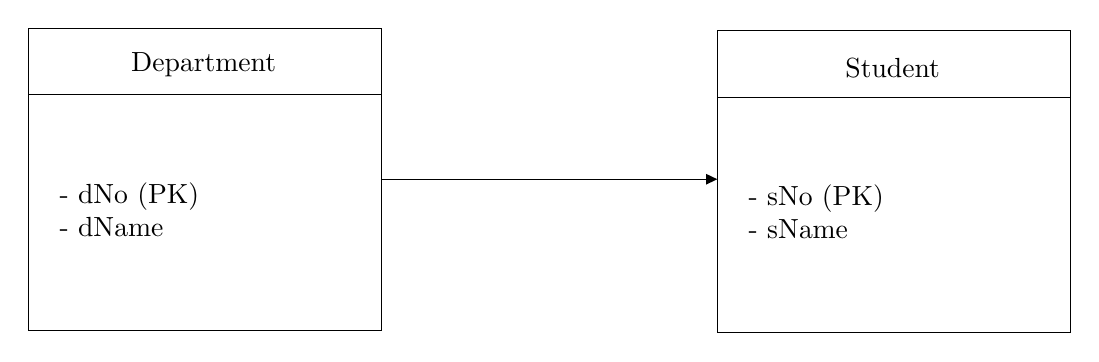
\begin{tikzpicture}[x=0.75pt,y=0.75pt,yscale=-1,xscale=1]
    %uncomment if require: \path (0,300); %set diagram left start at 0, and has height of 300

    %Shape: Rectangle [id:dp07523731865033279] 
    \draw   (87,100) -- (257,100) -- (257,245.5) -- (87,245.5) -- cycle ;
    %Straight Lines [id:da3910203522703485] 
    \draw    (87,132) -- (257,132) ;

    %Straight Lines [id:da8499453457607233] 
    \draw    (257,172.75) -- (416,172.75) ;
    \draw [shift={(419,172.75)}, rotate = 180] [fill={rgb, 255:red, 0; green, 0; blue, 0 }  ][line width=0.08]  [draw opacity=0] (5.36,-2.57) -- (0,0) -- (5.36,2.57) -- cycle    ;
    %Shape: Rectangle [id:dp9006099344965471] 
    \draw   (419,101.25) -- (589,101.25) -- (589,246.75) -- (419,246.75) -- cycle ;
    %Straight Lines [id:da5642236534532944] 
    \draw    (419,133.25) -- (589,133.25) ;


    % Text Node
    \draw (171.5,187.25) node   [align=left] {\begin{minipage}[lt]{104.04pt}\setlength\topsep{0pt}
    \mbox{-} dNo (PK)\\\mbox{-} dName
    \end{minipage}};
    % Text Node
    \draw (171.5,117.75) node   [align=left] {\begin{minipage}[lt]{106.76pt}\setlength\topsep{0pt}
    \begin{center}
    Department
    \end{center}

    \end{minipage}};
    % Text Node
    \draw (503.5,119) node   [align=left] {\begin{minipage}[lt]{106.76pt}\setlength\topsep{0pt}
    \begin{center}
    Student
    \end{center}

    \end{minipage}};
    % Text Node
    \draw (503.5,188.5) node   [align=left] {\begin{minipage}[lt]{104.04pt}\setlength\topsep{0pt}
    \mbox{-} sNo (PK)\\\mbox{-} sName
    \end{minipage}};


    \end{tikzpicture}
\caption{}
\end{figure}

\chapter{关系模式规范化理论}

\begin{example}
    现有关系模式: $R(A, B, C, D, E)$, 存在函数依赖 
    $A B C \rightarrow D E, A C \rightarrow D, D \rightarrow E$.
    问:
    \begin{enumerate}[label={$\left.\arabic*\right)$}, itemsep=0pt]
        \item 关系 $R$ 属于第几范式? 
        \item 若关系 $R$ 不属于 $B C N F$, 请将其逐步分解为 BCNF.
    \end{enumerate}
    要求写出每一级范式的分解过程。
\end{example}

\begin{example}
    现有关系模式: $R(A, B, C, D, E, F)$,
    存在函数依赖 
    $B \rightarrow C, A \rightarrow D, 
    A B \rightarrow E, D \rightarrow F$. 问:
    \begin{enumerate}[label={$\left.\arabic*\right)$}, itemsep=0pt]
        \item 关系 $R$ 属于第几范式?
        \item 若关系 $R$ 不属于 $B C N F$, 请将其逐步分解为 BCNF.
    \end{enumerate}
    要求写出每一级范式的分解过程。
\end{example}

\appendix
% 设置 chapter 标题样式
\titleformat{\chapter}[hang]{\centering\heiti\Large\bfseries}{附录\,\thechapter}{1em}{}
\renewcommand{\chaptermark}[1]{\markboth{附录 \thechapter\, #1}{}}

\chapter{集合论}

\section{公理化集合论}

接下来我们介绍一个公理系统, 该公理系统描述了被称为{\kaishu 集合}的数学对象的性质,
在介绍这些公理后, 我们将展示这些公理的一些最简单的推论.

\subsection{Zermelo-Fraenkel 公理系统}

\setcounter{axiom}{0}
\begin{axiom}[外延公理]
    $A = B \iff \forall x \left( (x \in A) \iff (x \in B) \right)$, 
    即集合 $A$ 与集合 $B$ 相等, 当且仅当它们所具有的各元素是相同的.
\end{axiom}
\begin{axiom}[分离公理]
    集合 $A$ 和性质 $P$ 总能够确定一个集合 $B$, 
    其元素是且仅是 $A$ 中具有性质 $P$ 的元素,
    即 $B = \left\{ x \in A | P(x) \right\}$.
\end{axiom}

\begin{example}
    我们可以用分离公理来理解差集运算, 设 $A,B$ 是两个集合, $A \setminus B
    \xlongequal{\mathrm{def}} \left\{ x \in A | x \notin B \right\}$,
    显然这里的 $A$ 是一个集合, 而 $x \notin B$ 是一个性质, 它们总是能够确定
    这样的集合 $A \setminus B$.
\end{example}
\begin{example}
    试证明 {\kaishu $\forall A \left( \varnothing \in A \right)$, 即空集是任何集合的
    子集}.
    \begin{proof}
        分离公理在一些数学结构中是很常用的, 我们需要从一个集合 $A$ 中分离出具有性质
        $P$ 的元素来. 显然, 在这个问题中, 设 $X$ 是一个集合, 那么我们能够分离出它的
        空子集 $\varnothing_X = \left\{ x \in X | x \ne x \right\}$ 来.
        设 $Y$ 是另一个任意给定的集, 有 $\varnothing_Y = \left\{ y \in Y |
        y \ne y \right\}$, 根据外延公理, $\varnothing_X = \varnothing_Y$.
        由于我们的 $X,Y$ 都是任意给定的集合, 这就是说, 空集是唯一的, 我们用 $\varnothing$
        来表示空集, 并且, 任何集合都有空子集.
    \end{proof}
\end{example}

\begin{axiom}[并集公理]
    由集合族 $\mathscr{A}$ 的诸集合 $A_i$ 的元素组成的集合 
    $\cup \mathscr{A}$ 是存在的. 即集合的并集是一个集合, 且
    \[ x \in \cup \mathscr{A} \iff \exists A \in \mathscr{A} \left(
        x \in A
    \right). \]
\end{axiom}

\begin{example}
    根据并集公理和分离公理, 我们可以给出集合族 $\mathscr{A}$ 的交集 $\cap \mathscr{A}$
    的定义, 并集概念的核心是并集中的元素属于集合族中的每一个集合, 因此 
    $\cap \mathscr{A} \xlongequal{\mathrm{def}} \left\{ x \in \cup 
    \mathscr{A} | \forall A \in \mathscr{A} (x \in A) \right\}$.
\end{example}

\begin{axiom}[配对公理]
    对于集合 $X$ 和集合 $Y$, 存在一个集合, 其元素是且仅是 $X$ 和 $Y$, 
    将该集合记作 $\left\{ X,Y \right\}$, 
    称为集合 $X,Y$ 的{\normalfont\bfseries 无序偶}.
\end{axiom}

\begin{axiom}[子集之集公理]
    对于任意给定的集合 $A$, 存在一个集合 $\mathscr{P}(A)$, 使得 $\mathscr{P}(A)$
    中的元素是且仅是 $A$ 的子集, 即 
    $\mathscr{P}(A) = \left\{ X | X \subset A \right\}$.
\end{axiom}

\begin{example}
    现在我们来回答为什么要按照定义 \ref{def: 二元关系} 的方式来定义二元关系.
    T.B.C. \label{TBC}
\end{example}

公理 $1 \sim 5$ 限制了形成新集合的可能性.
为了表述下面的公理, 我们需要给定后继集和归纳集的概念.

\begin{definition}[后继集]
    设 $X$ 是一个集合, 集合 $X \cup \left\{ X \right\}$ 称为 $X$ 的\textbf{后继集},
    即在 $X$ 中补充一个单元素集合 $\left\{ X \right\}$. 集合 $X$ 的后继集记作
    $X^+$.
\end{definition}
\begin{definition}[归纳集]
    假设 $X$ 是一个集合, 如果 $X$ 包含空集以及自身任何一个元素的后继集, 则称 $X$
     是一个归纳集.
\end{definition}

\begin{axiom}[无穷公理]
    归纳集, 即{\bfseries 包含空集以及自身任何一个元素的后继集}的集合, 是存在的.
\end{axiom}

\begin{example}
    根据无穷公理和公理 $1 \sim 4$, 我们可以建立自然数集 $\mathbb{N}_0$ 的 Von 
    Neumann 方案. 我们把自然数集 $\mathbb{N}_0$ 定义为各归纳集的交集, 即最小归纳集.
    $\mathbb{N}_0$ 的元素是集合
    \[ \varnothing, \varnothing^+, \left( \varnothing^+ \right)^+, \]
    其中, $\varnothing^+ = \varnothing \cup \left\{ \varnothing \right\}
    = \left\{ \varnothing \right\}$, 而 $\left\{ \varnothing \right\}^+
    = \left\{ \varnothing \right\} \cup \left\{ 
        \left\{ \varnothing \right\}
    \right\}$. 这些集合就是我们用符号 $0,1,2,\cdots$ 表示的并称之为自然数的
    数学对象的模型.
\end{example}

\onecolumn
\begin{thebibliography}{1}
    \addcontentsline{toc}{chapter}{参考文献}
    \bibitem{数据库系统基础}
    [美] Rames Elmasri, [美] Shamkant B. Navathe. 数据库系统基础: 第 7 版
    (Fundamentals of Database Systems, 7e)[M].
    陈宗斌等译. 北京: 清华大学出版社, 2020.
    \bibitem{zorich}
    [俄罗斯] B.A.Zorich. 数学分析: 第 7 版. 第一卷[M].
    北京: 高等教育出版社, 2019
\end{thebibliography}

\newpage
\thispagestyle{empty}
\vspace*{5cm}
\begin{center}
    \includegraphics*[width=\textwidth]{pic/i_love_npu.jpeg}
    \large
    公诚勇毅 \quad 永矢毋忘

    中华灿烂 \quad 工大无疆
\end{center}
\vspace*{13em}
\begin{center}
    \small
    本文档由\textbf{钱锋}编写, 钱锋保留一切权利.

    文档中出现的部分素材来源于网络, 笔者承诺这些素材仅供学习交流之用, 
    它们的原作者保留一切权利.

    2023 年 \quad 西北工业大学 \quad 中国西安 
\end{center}

\end{document}